\documentclass[12pt,letterpaper]{article}
\usepackage[utf8x]{inputenc}
\usepackage{ucs}
\usepackage[spanish]{babel}
\usepackage{amsmath}
\usepackage{amsfonts}
\usepackage{amssymb}
\usepackage{graphicx}
\usepackage[left=0.5cm,right=0.5cm,top=0.5cm,bottom=0.5cm]{geometry}
\author{F\'elix Ernesto Charry Pastrana}
\sloppy
\setlength{\parindent}{0pt}
\usepackage[none]{hyphenat}
\begin{document}
\textbf{Universidad Nacional Autónoma de México }\\
Presentado por: \textbf{F. E. Charry-Pastrana}\\
Presentado a: \textbf{Santiago Caballero} \\
Posgrado en Ciencias Físicas \\
Introducción a Física Computacional \\
2018.04.19 \\
\\
\textbf{{\Large Tarea: Solución de ecuaciones diferenciales mediante Runge-Kutta. \textit{Comparación de diferentes métodos y oscilador armónico}}}
\begin{figure}[h]
\centering
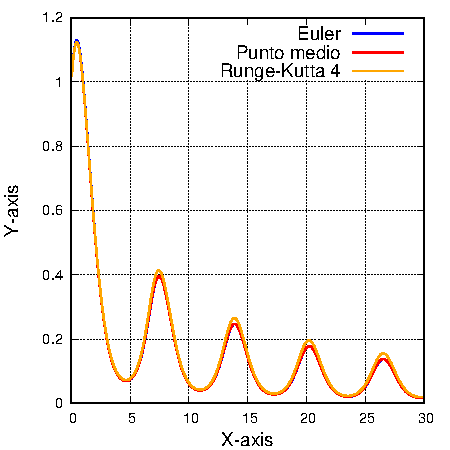
\includegraphics[width=0.75\textwidth]{Parte_A.pdf}
\caption{Comparación entre diferentes métodos para la solución de la ecuación diferencial $\dfrac{dy}{dx} = y\,\cos(x+y)$.}
\end{figure}

\begin{figure}
\centering
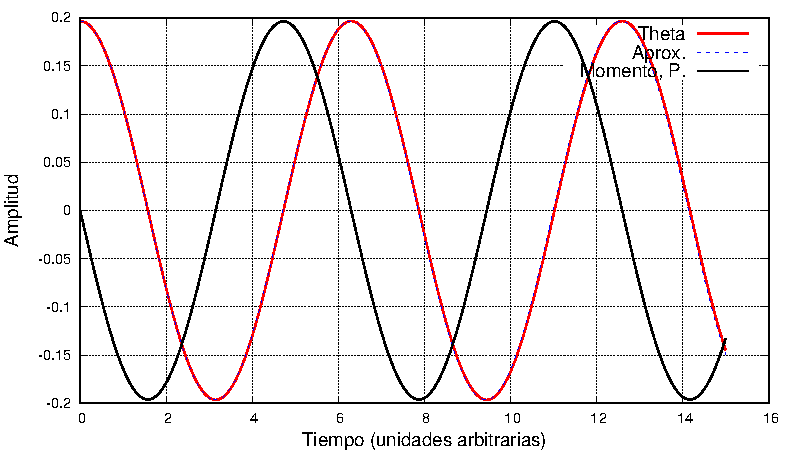
\includegraphics[width=0.95\textwidth]{Pi16P0.pdf}
\caption{Oscilador armónico con condiciones iniciales: $\theta_0 = \dfrac{\pi}{16}$ y $P_{\theta,0} =  0$}
\end{figure}
\begin{figure}
\centering
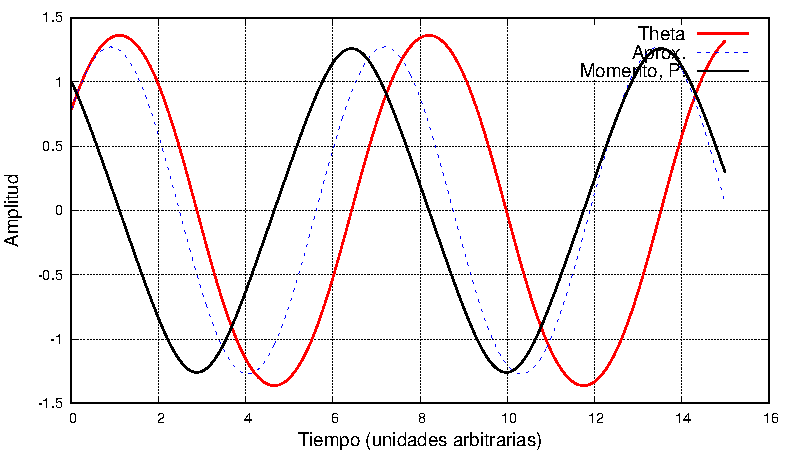
\includegraphics[width=0.95\textwidth]{Pi4P1.pdf}
\caption{Oscilador armónico con condiciones iniciales: $\theta_0 = \dfrac{\pi}{4}$ y $P_{\theta,0} =  1$}
\end{figure}
\begin{figure}
\centering
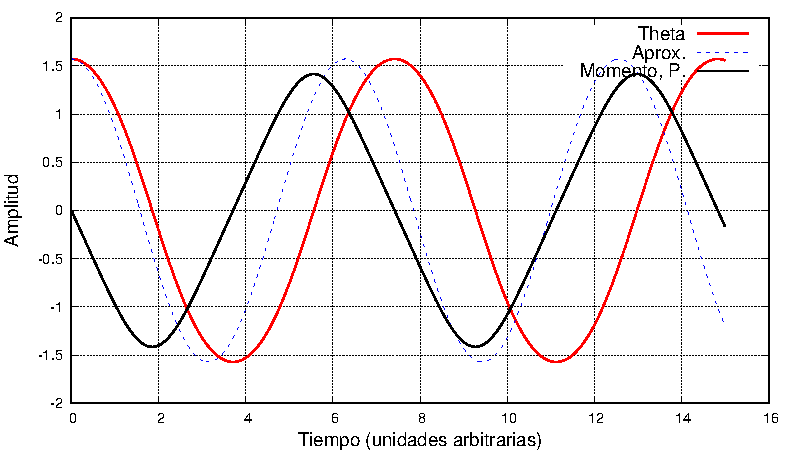
\includegraphics[width=0.95\textwidth]{Pi2P0.pdf}
\caption{Oscilador armónico con condiciones iniciales: $\theta_0 = \dfrac{\pi}{2}$ y $P_{\theta,0} =  0$}
\end{figure}
\begin{figure}
\centering
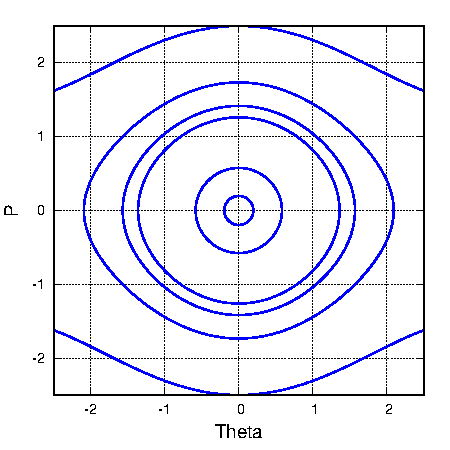
\includegraphics[width=0.95\textwidth]{Phase_Space.pdf}
\caption{Espacio Fase}
\end{figure}
\begin{figure}
\centering
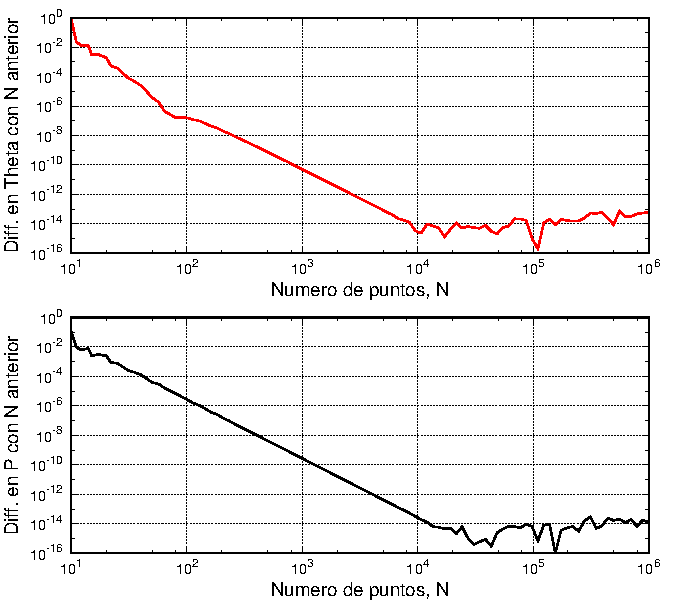
\includegraphics[width=0.95\textwidth]{Dep_N.pdf}
\caption{Diferencia entre valor de $\theta$ o $P_{\theta}$ para el tiempo $t=10$ respecto al valor para $N$ anterior. Las condiciones iniciales en todos los casos fueron: $\theta_0 = \dfrac{\pi}{4}$ y $P_{\theta,0} =  1$}
\end{figure}
\end{document}